\section{Stima temporale del progetto}
\label{sec:stima_temporale}

\par Il calendario di massima è suddiviso in due revisioni di avanzamento, identificate rispettivamente con le abbreviazioni \glossario{RTB} (Requirements and Technology Baseline) e \glossario{PB} (Product Baseline). Nonostante sia stata effettuata un'analisi preliminare dei rischi e delle attività, le date stimate durante la stesura iniziale del \PdP\ sono soggette a variazioni. Ciascuno \glossario{sprint}, infatti, presenta una sezione denominata consuntivo, il cui scopo, tra gli altri, è quello di aggiornare le stime temporali in base all'andamento effettivo del progetto.

\subsection{Ultimo aggiornamento: 2024-07-10}
\begin{figure}[H]
  \centering
  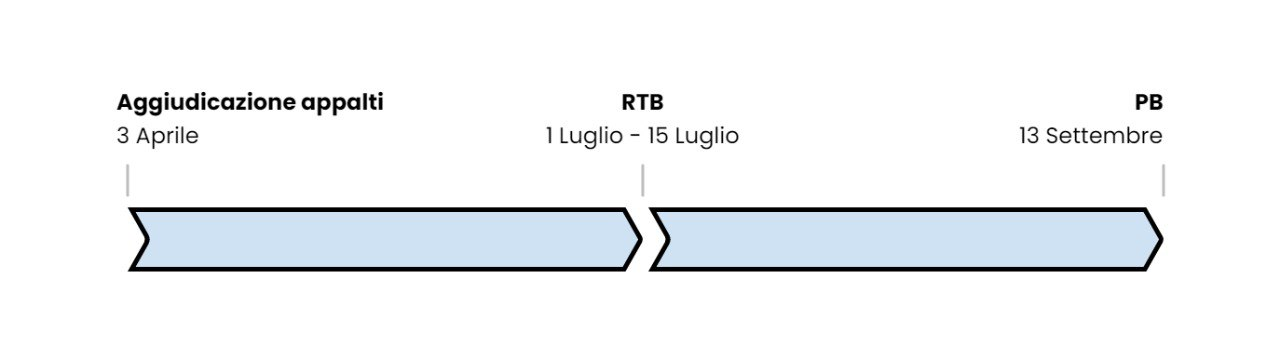
\includegraphics[width=\textwidth]{assets/stimatemporale.png}
  \caption{Stima temporale delle revisioni di progetto}\label{fig:stima-temporale}
\end{figure}
